\documentclass[a4paper, 12pt]{article}

\usepackage{geometry}
\geometry{left=2cm, right=2cm, top=2cm, bottom=2cm}
\usepackage{wrapfig}
\usepackage{cmap}
\usepackage{mathtext} 
\usepackage[T2A]{fontenc}
\usepackage[utf8]{inputenc}
\usepackage[english,russian]{babel}	

\usepackage{amsfonts,amssymb,amsthm,mathtools}
\usepackage{amsmath}
\usepackage{icomma} 

\usepackage{graphicx} 
\graphicspath{{picturies/}}
\usepackage{wrapfig}

\usepackage{array,tabularx,tabulary,booktabs}
\usepackage{longtable}
\usepackage{multirow}

\usepackage{caption}
\captionsetup{labelsep=period}

\renewcommand{\phi}{\varphi}
\newcommand{\eps}{\varepsilon}
\newcommand{\parag}[1]{\paragraph*{#1:}}
\newcommand{\mysec}[1]{\begin{center}\section*{#1}\end{center}}

\author{Радькин Кирилл Б01-005}
\title{3.4.1. Диа- и парамагнетики}
\date{8.10.21}

\graphicspath{{pictures/}}


\begin{document}

\maketitle

\parag {Цель работы} измерение магнитной восприимчивости диа- и парамагнитного образа.

\parag {В работе используются} электромагнит, аналитические весы, миливеберметр, амперметр постоянного тока, реостаты, образцы.
\\

Магнитная восприимчивость тел может быть определена методом измерения сил, которые жействуют на тела в магнитном поле. 
Существуют два классических метода таких измерений: \textit{метод Фарадея и метод Гюи}. 
В методе Фарадея исследуемые образцы, имеющие форму маленьких шариков, помещаются в область сильно неоднородного магнитного поля и измеряется сила, действующая на образец. 
При этом для расчета магнитной восприимчивости необходимо знать величину градиентного магнитного поля в месте расположения образца. 
В методе Гюи используется тонкий и длинный стержень, один из концов которого помещают в зазор электромагнита (обычно в область однородного поля), а другой конец~---~вне зазора, где величиной магнитного поля можно пренебречь. 
Закон изменения поля~---~от максимального до нулевого в этом случае несущественен.
\\

\begin{wrapfigure}{l}{0.3\linewidth}
    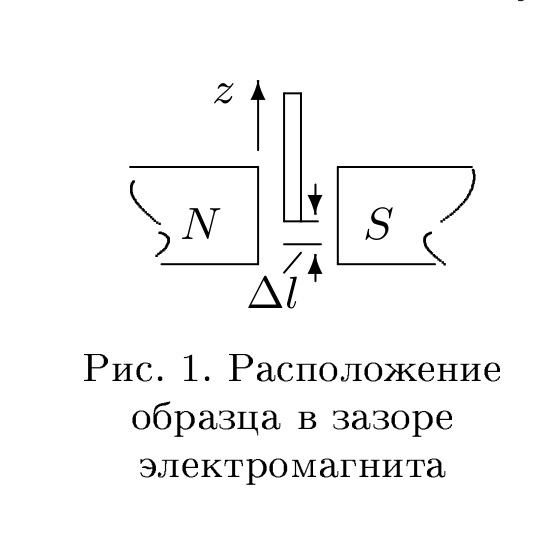
\includegraphics[scale=0.2]{pic1.jpg}
\end{wrapfigure}

Найдем выражение для магнитной силы, действующей на такой образец (рис. 1). 
Пусть площадь образца равна $s$, его магнитная проницаемость~---~$\mu$, а поле в зазоре равно $B$.
\\

Воспользуемся для расчета энергетическими соображениями. 
Магнитная сила может быть вычислена как производная от магнитной энергии по перемещению. 
Из теории известно, что эту производную следует брать со знаком минус, когда образец находится в поле постоянного магнита, или со знаком плюс, как в нашем случае, когда поле в зазоре создается электромагнитом, ток $I$ в обмотках которого поддерживается постоянным.
\\

При смещении образца на расстояние $\Delta l$ вниз магнитная сила, действующая на него равна

\begin{equation}
    F = \left( \dfrac{\Delta W_m}{\Delta l}_I \right), 
\end{equation}

где $\Delta W_m$~---~изменение магнитной энергии системы при постоянном токе в обмотке электромагнита и, следовательно, при постоянной величине магнитного поля в зазоре.
\\

Магнитная энергия рассчитывается по формуле

\begin{equation}
    W_m = \dfrac{1}{2} \int H B  dV = \dfrac{1}{2 \mu_0} \int \dfrac{B^2}{\mu} dV
\end{equation}

где интеграл распространен на все пространство. 
При смещении образца магнитная энергия меняется только в области зазора (в объеме площади $s$ и высоты $\Delta l$), а около верхнего конца стержня остается неизменной, поскольку магнитного поля там практически нет. 
Принимая поле внутри стержня равным измеренному нами полю в зазоре B, получим

\begin{equation*}
    \Delta W_m = \dfrac{1}{2\mu_0} \dfrac{B^2}{\mu} s \Delta l - \dfrac{1}{2 \mu_0}B^2 s \Delta l = \dfrac{1 - \mu}{2 \mu_0 \mu} B^2 s \Delta l = -\dfrac{\chi}{2 \mu_0 \mu}B^2 s \Delta l
\end{equation*}

Следовательно, на образец действует сила

\begin{equation}
    F = - \dfrac{\chi}{2 \mu_0 \mu} B^2 s
\end{equation}

Знак силы, действующей на образец зависит от знака $\chi$: образцы из парамагнитных материалов ($\chi > 0$) втягиваются в зазор электромагнита, а диамагнитные образцы ($\chi < 0$) выталкиваются из него.
\\

Пренебрегая отличием $\mu$ от единицы, получаем окончательно расчетную формулу в виде

\begin{equation}
    F = - \dfrac{\chi B^2 s}{2 \mu_0}
\end{equation}

Измерив силу, действующую на образец в магнитном поле $B$, можно рассчитать магнитную восприимчивость образца.

\begin{center}
    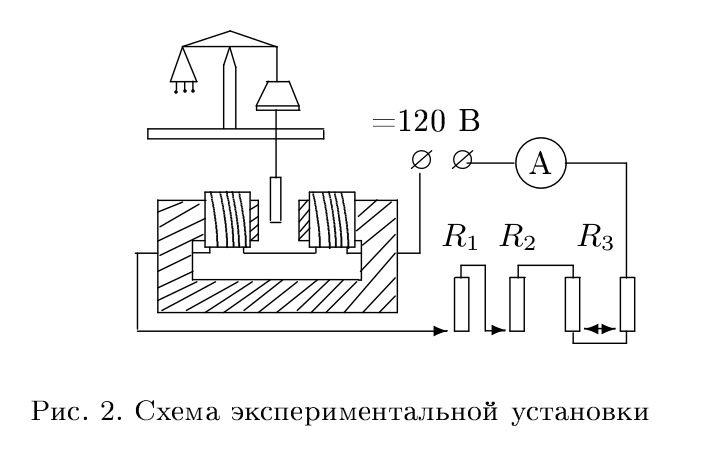
\includegraphics[scale=0.4]{pic2.jpg}    
\end{center}

\parag{Экспериментальная установка}

Схема установки изображена на рис. 2. 
Магнитное поле с масимальной индукцией $\simeq 1.5 Тл$ создается в зазоре электромагнита, питаемого постоянным током. 
Диаметр полюсов существенно превосходит ширину зазора, поэтому поле в средней части зазора достаточно однородно. 
Величина тока, проходящего через обмотки электромагнита, регулируется при помощи трез реостатов $R_1, R_2, R_3$  и измеряется многопредельным амперметром $A$. 
Тонкая проволока высокоомных реостатов не рассчитана на большой ток, поэтому регулировку более низкоомными реостатами следует проводить только при \textbf{полностью} выведенных высокоомных реостатах.
\\
Градуировка электромагнита (связь между индукцией магнитного поля $B$ в зазоре электромагнита и силой тока $I$ в его обмотках) производится при помощи милливебметра.
\\
При измерениях образцы поочередно подвешиваются к аналитическим весам так, что один конец обращца оказывается в зазоре электромагнита, а другой~---~вне зазора, где индукцией магнитного поля можно пренебречь. 
При помощи аналитических весов определяется перегрузка $\Delta P=F$~---~сила, действующая на образец со стороны магнитного поля.
\\
Как уже отмечалось, силы, действующие на диа- и парамагнетные образцы очень малы.
Небольшие примеси ферромагнетиков (сотые доли процента железа и никеля) способны кардинально изменить результат опыта, поэтому образцы были специально отобраны.

\mysec{Задание}

В работе предлагается исследовать зависимость силы, действующей на образец, размещенный в зазоре электромагнита, от величины поля в зазоре и по результатам измерений рассчитать магнитную восприимчивость меди и алюминия.

\begin{enumerate}
    \item Проверим работу цепи питания электромагнита. Оценим диапазон тока $I$ через обмотки: $I \leq 3.02 A$
    
    \item Прокалибруем электромагнит. 
    Для этого с помощью милливебметра снимем зависимость магнитного потока $\Phi$, пронизывающего пробную катушку, находящуюся в зазоре от тока $I$ ($\Phi = BSN$). 
    Значение $SN = 72 см^2$ (произведение площадей сечения пробной катушки на число витков в ней) указано на установке.

    \item Убедимся, что весы арретированы.
    
    \item Измерим силы (изменение показаний весов), действующие на образец в магнитном поле.
    \\\\
    Медь:
    \\
    \begin{tabular}{|c|c|c|c|c|c|} \hline
        $dm, г$ & 0 & -0.001 & -0.002 & -0.002 & -0.005 \\ \hline
        $I, A$ & 0.3 & 0.6 & 0.9 & 1.2 & 1.5\\ \hline
        $dm, г$ &-0.008 & -0.011 & -0.014 & -0.017 & -0.02 \\ \hline
        $I, A$ & 1.8 & 2.1 & 2.4 & 2.7 & 3 \\ \hline
    \end{tabular}
    \\\\
    Алюминий:
    \\
    \begin{tabular}{|c|c|c|c|c|c|} \hline
        $dm, г$ & 0.001 & 0.002 & 0.005 & 0.01 & 0.014 \\ \hline
        $I, A$ & 0.3 & 0.6 & 0.9 & 1.2 & 1.5 \\ \hline
        $dm, г$ & 0.019 & 0.025 & 0.032 & 0.039 & 0.045 \\ \hline
        $I, A$ & 1.8 & 2.1 & 2.4 & 2.7 & 3 \\ \hline
    \end{tabular}
    \\\\
    Графит:
    \\
    \begin{tabular}{|c|c|c|c|c|c|} \hline
        $dm, г$ & 0.014 & 0.043 & 0.079 & 0.114 & 0.153 \\ \hline
        $I, A$ & 0.3 & 0.6 & 0.9 & 1.2 & 1.5 \\ \hline
        $dm, г$ & 0.194 & 0.238 & 0.281 & 0.317 & 0.344 \\ \hline
        $I, A$ & 1.8 & 2.1 & 2.4 & 2.7 & 3 \\ \hline
    \end{tabular}
\end{enumerate}

\mysec{Обработка результатов}
\begin{enumerate}
    \item Рассчитаем поле $B$ и построим градуировочную кривую для электромагнита: $B = f \left( I \right)$
    \\
    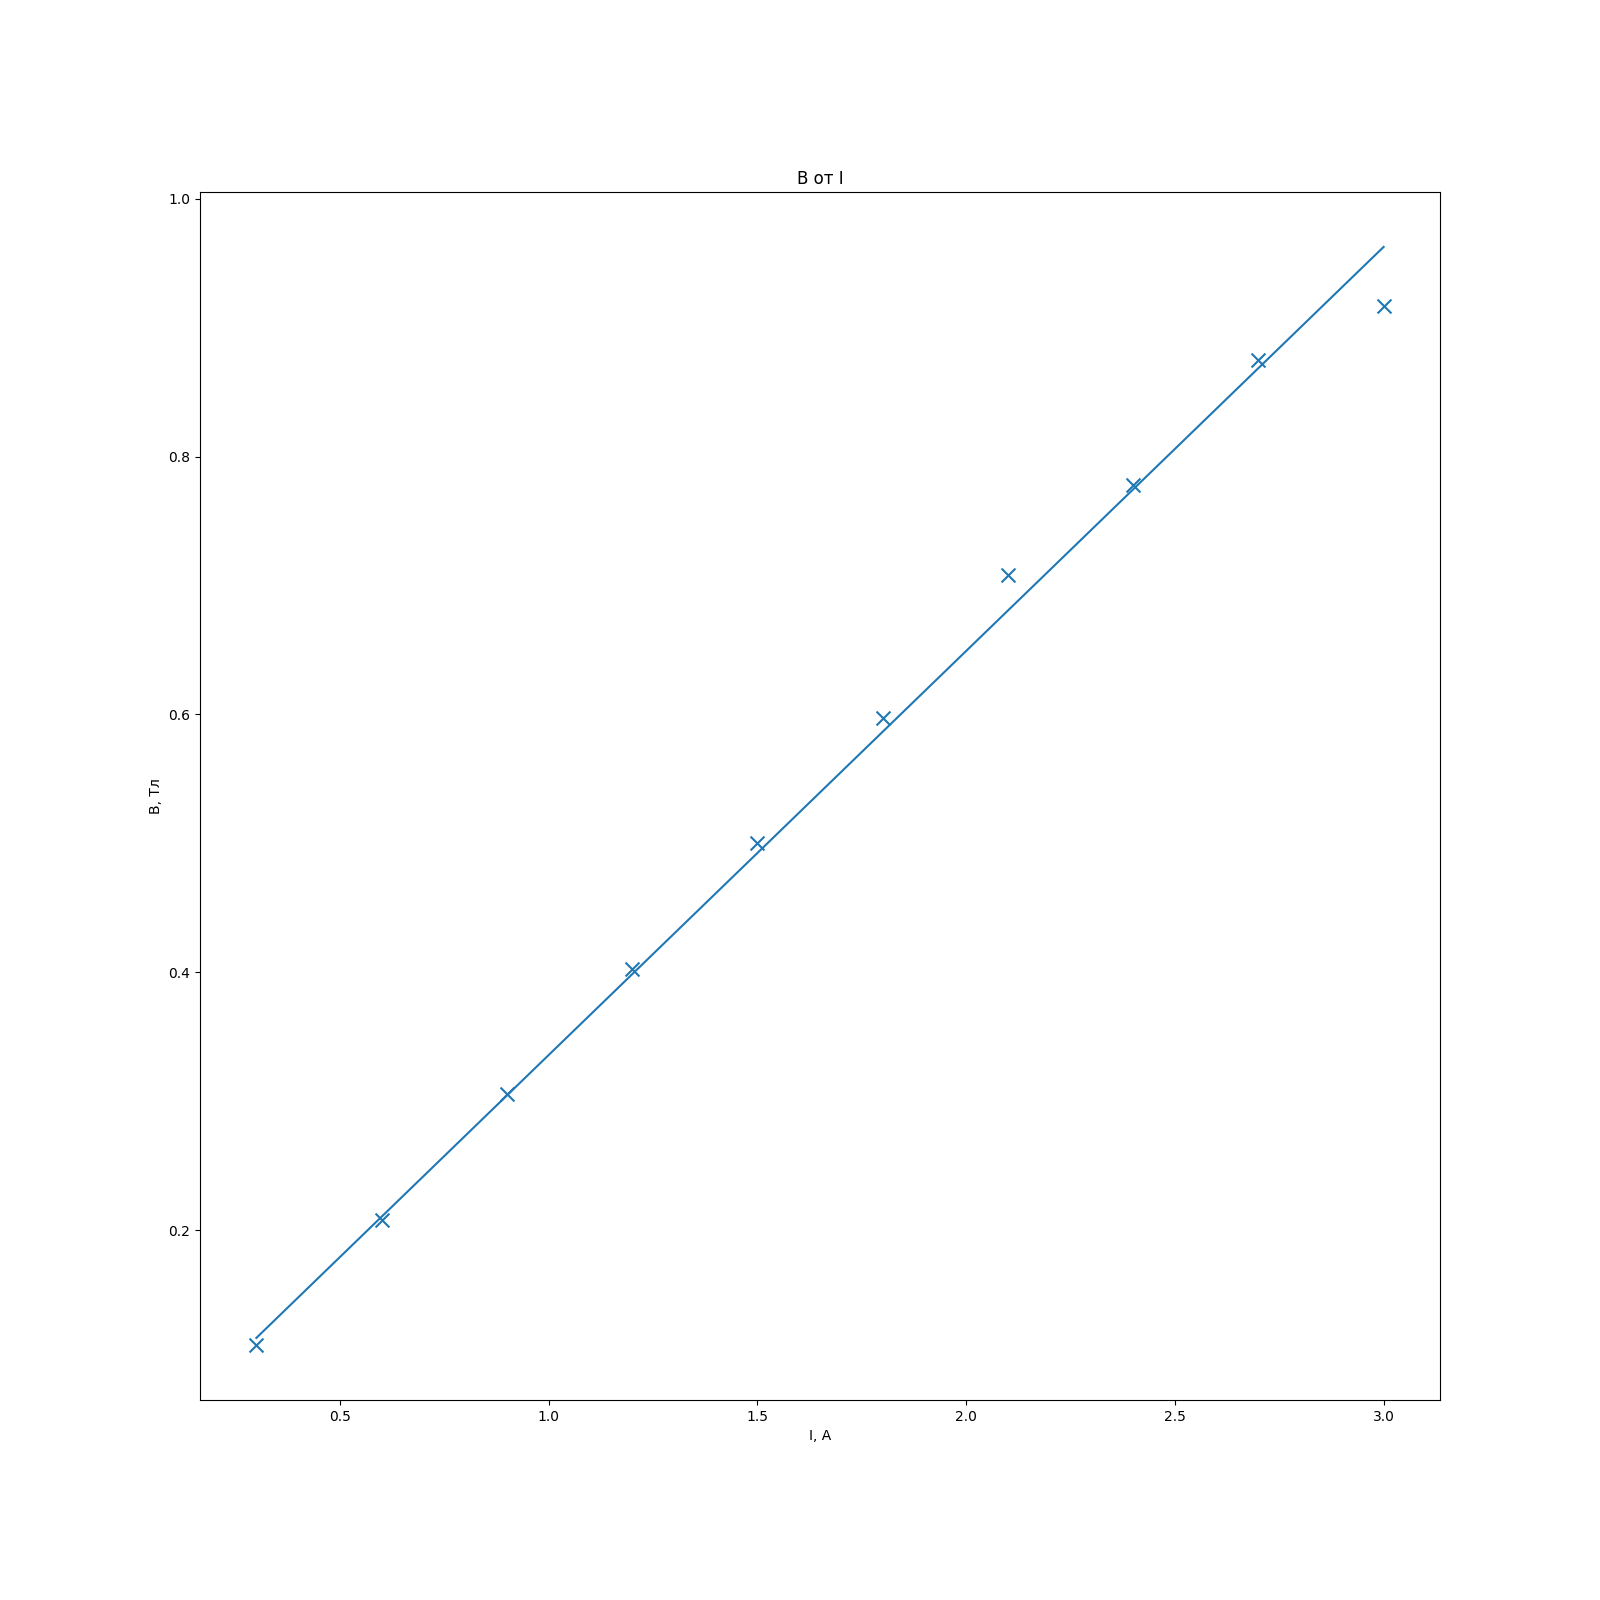
\includegraphics[width=\linewidth]{graph1.png}

    \item Построим графики $|\Delta P| = f(B^2)$ для меди, алюминия и графита.
    
    \item По наклонам полученных прямых рассчитаем величину $\chi$ с помощью формулы (4):
    \\\\
    $\chi_{меди} = (-5.78 \pm 0.38) \cdot 10^{-6} \text{ } \dfrac{1}{моль}$ 
    \\\\
    $\chi_{ал} = (1.67 \pm 0.08) \cdot 10^{-5} \text{ } \dfrac{1}{моль}$
    \\\\
    $\chi_{гр} = (2.87 \pm 0.14) \cdot 10^{-4}$ (неизвестна масса графитового стержня)

    \item Сравним с табличными (с учетом массы): 
    \\\\
    $\chi_{меди} = -5.41 \cdot 10^{-6} \dfrac{1}{моль}$
    \\\\
    $\chi_{алюминия} = 2.3 \cdot 10^{-5} \dfrac{1}{моль}$

    \item Вывод. Для меди значения почти совпали с табличными, для алюминия отличие примерно на $50 \%$, для графита сравнить не удалось.

    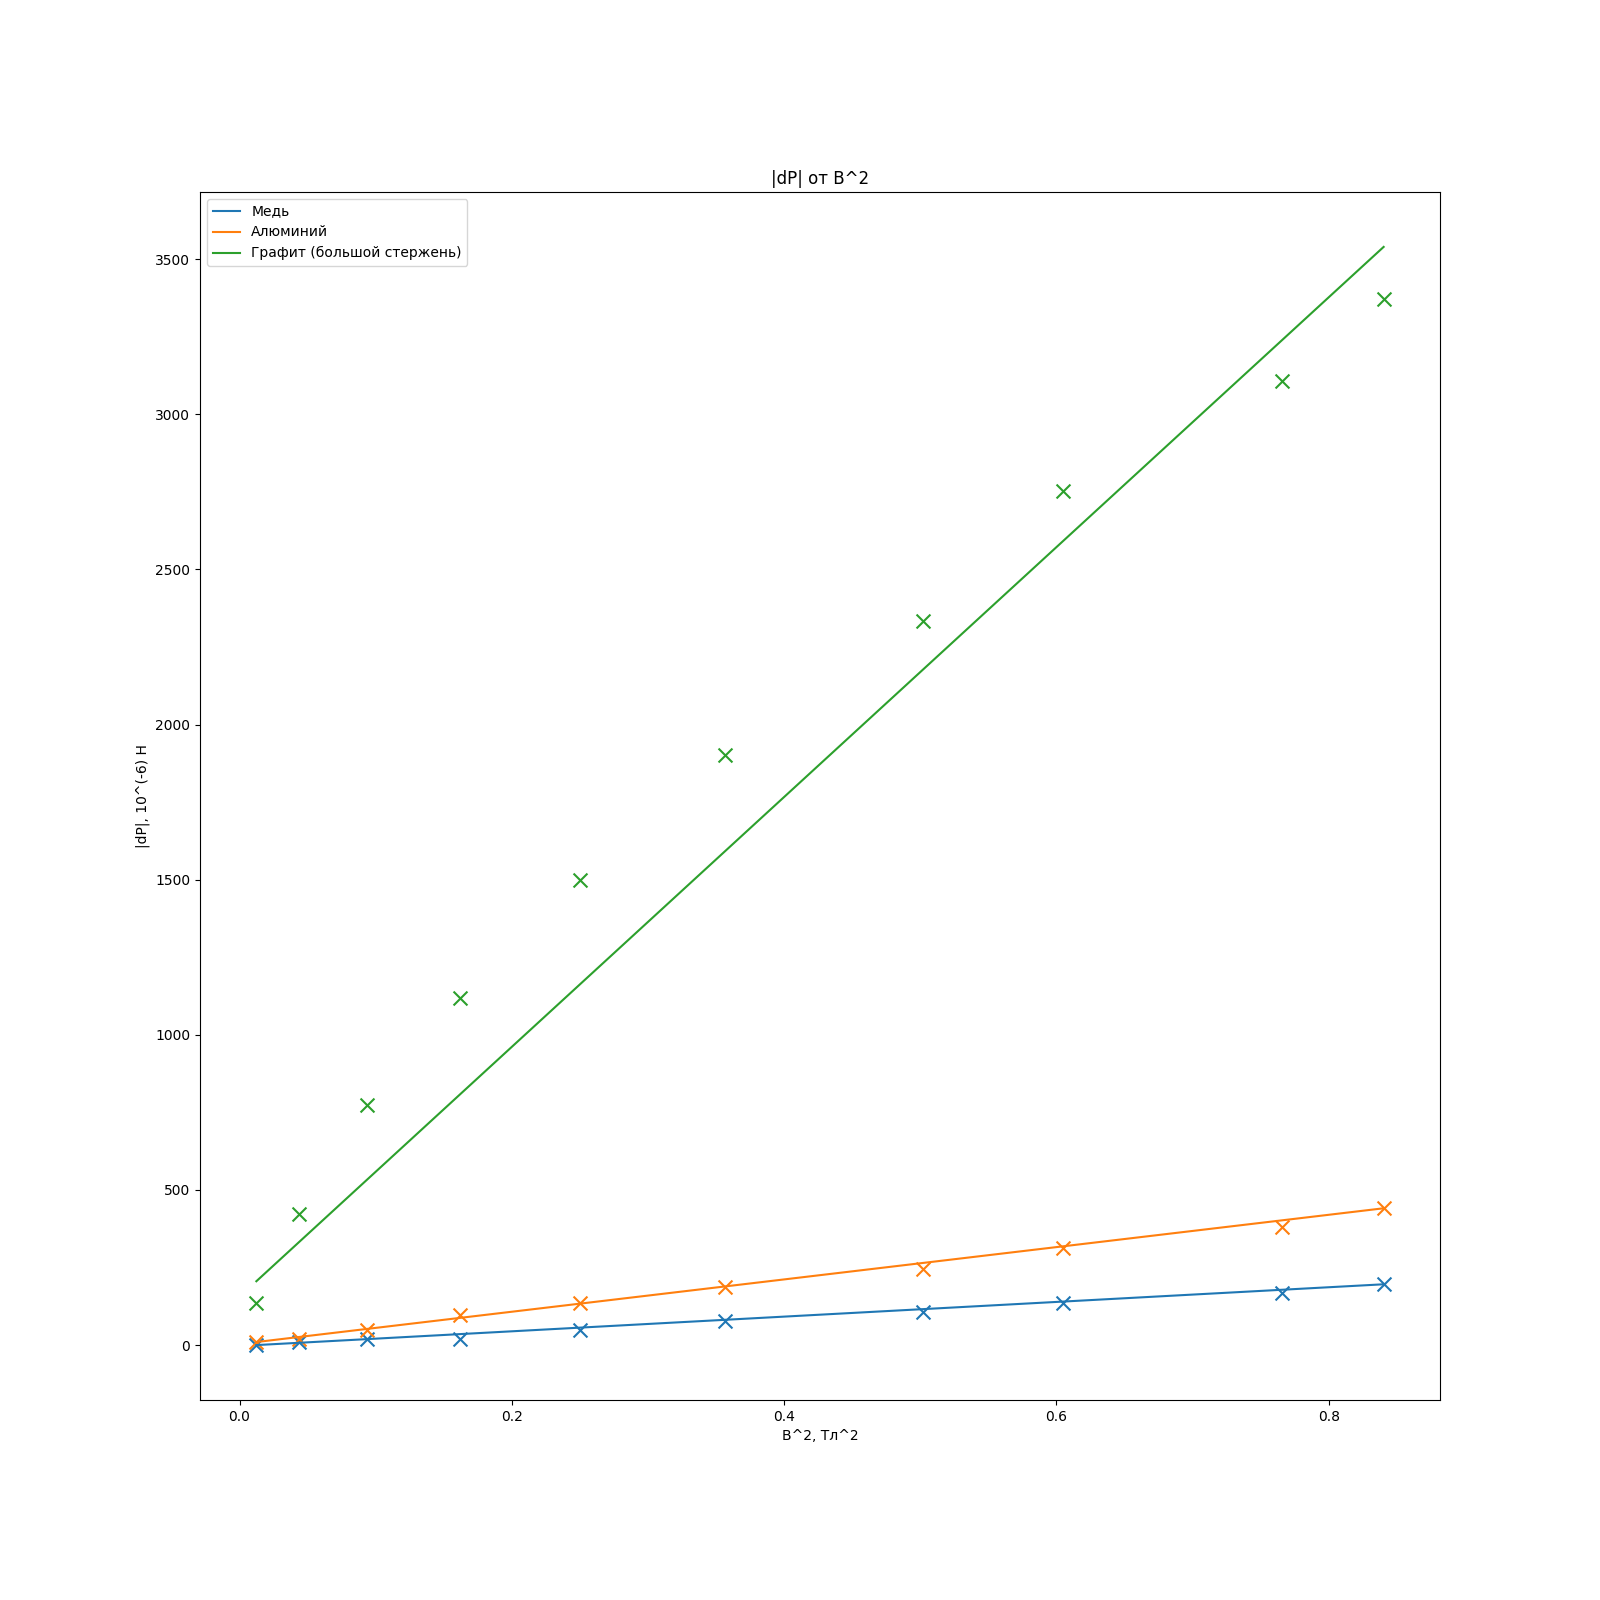
\includegraphics[width=\linewidth]{graph2.png}
\end{enumerate}

\end{document}
